

\chapter{Overview dell'architettura e delle componenti utilizzate}

\label{ch:overview}

\section{Obbiettivo da ottenere}

In una collaborazione tra il Dipartimento di Ingegneria dell'Informazione e l'azienda \textbf{Esse-ti S.R.L.} ci è stato esposto un progetto che consiste nel:

%todo non mi piace come sta messo
\begin{itemize}
	\item fornire a dei clienti un router 4G, su cui possono essere connessi vari dispositivi, ad es. di tipo domotico.
	\item rendere questi dispositivi accessibili ai clienti attraverso internet
\end{itemize}

\begin{figure}[H]
	\centering
	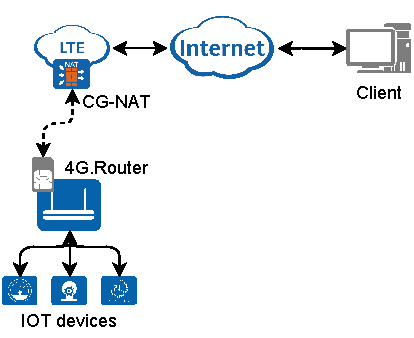
\includegraphics[width=0.5\linewidth]{immagini/diag-goal}
	\caption{Schema concettuale dell'obbiettivo da raggiungere. \cite{icons}}

	\label{fig:schema_concettuale}

\end{figure}

Data la presenza del CG-NAT si vede subito che non è realizzabile a meno che il cliente non abbia un'IP pubblico e la sua macchina venga configurata opportunamente. Questo però non è possibile nel caso generale, quindi per risolvere efficacemente questa topologia si deve necessariamente introdurre una terza macchina provvista di IP pubblico e che funga da ponte tra il 4G.Router e il cliente.


\begin{figure}[H]
	\centering
	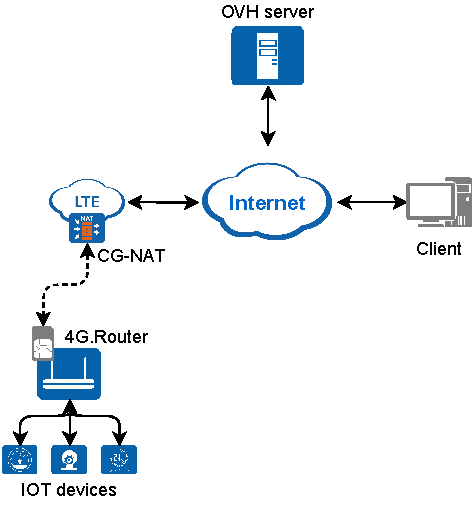
\includegraphics[width=0.5\linewidth]{immagini/diag-real}
	\caption{Schema concettuale dell'architettura che si dovrà implementare. \cite{icons}}

	\label{fig:schem_architettura_reale}

\end{figure}

%todo rivedi frase
In questo modo si può configurare una VPN sul server OVH e connettervi sia il 4G.Router che la macchina del cliente. In questo modo l'unica configurazione che il cliente dovrà fare è l'installazione di un cliente VPN, ciò è il minimo possibile di configurazione.

La configurazione virtuale vista dal 4G.Router e dai clienti sarà quindi:

\begin{figure}[H]
	\centering
	\includegraphics[width=0.5\linewidth]{immagini/diag-virtual}
	\caption{Topologia virtuale. \cite{icons}}

	\label{fig:schema_architettura_virtuale}

\end{figure}

% <-- section -->
\section{Specifiche dei componenti}

i componenti necessari sono:

\begin{itemize}
	\item Esse-ti 4G.Router
	\item Server
	\item Host domotico
	\item Macchina del cliente
\end{itemize}

vediamo le caratteristiche minime che i componenti dovranno avere:

\subsection{Esse-ti 4G.Router}

Ci è stato fornito dall'azienda Esse-ti, consiste in un gateway 4G con funzionalità di router. Le specifiche complete possono essere trovate sul sito del produttore (\href{https://www.esse-ti.it/4g-router}{link})


\begin{figure}[ht]
	\centering
	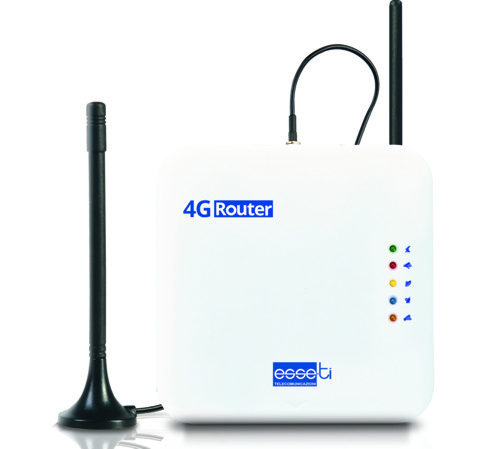
\includegraphics[width=250px]{immagini/4grouter.jpg}
	\caption{4G.Router}

	\label{fig:esse-ti-router-4g}

\end{figure}

Per l'implementazione di questa architettura sono necessarie solo un sub-set delle specifiche:

\begin{itemize} %TODO e' copiato e incollato va sistemato
	\item Access Point wireless per offrire connettività Internet Wi-Fi a dispositivi wireless
	\item Client Dynamic DNS per consentire all’utente di raggiungere da remoto, tramite Internet, il router stesso e tutti i dispositivi connessi via Wi-Fi o porta LAN
	\item Gateway telefonico per consentire l’invio e la ricezione di chiamate attraverso la rete 4G LTE/UMTS/GSM a telefoni fissi, combinatori o altri dispositivi telefonici collegati all’ingresso FXS
\end{itemize}

Presenta inoltre come sistema operativo una versione personalizzata di OpenWrt.

La configurazione del dispositivo puo' essere fatta sia da terminale, entrando in ssh, sia da interfaccia web:

\begin{figure}[H]

	\newlength{\tempheight}
	\setlength{\tempheight}{23ex}

	\centering%
	\begin{subfigure}[t]{0.5\textwidth}
		\centering%
		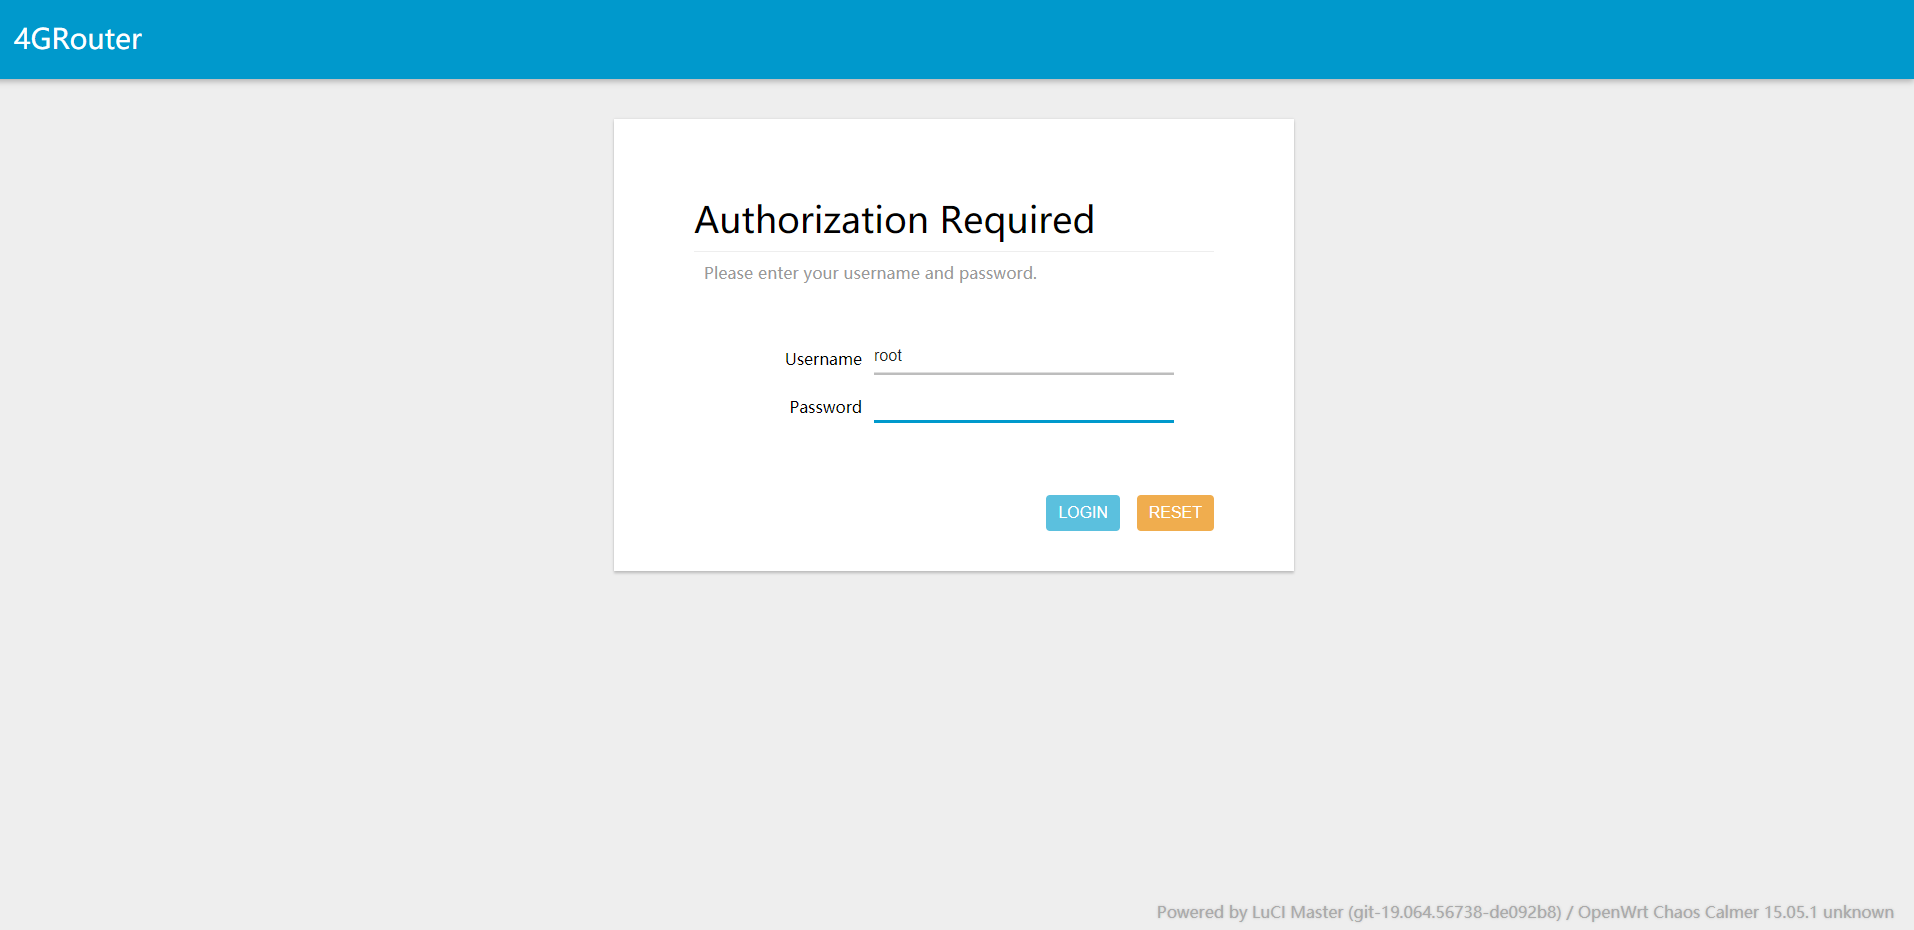
\includegraphics[totalheight=\tempheight]{immagini/interfacciar4g_init}
		\caption{Schermata di autenticazione}
	\end{subfigure}%
	\hfill
	\begin{subfigure}[t]{0.5\textwidth}
		\centering%
		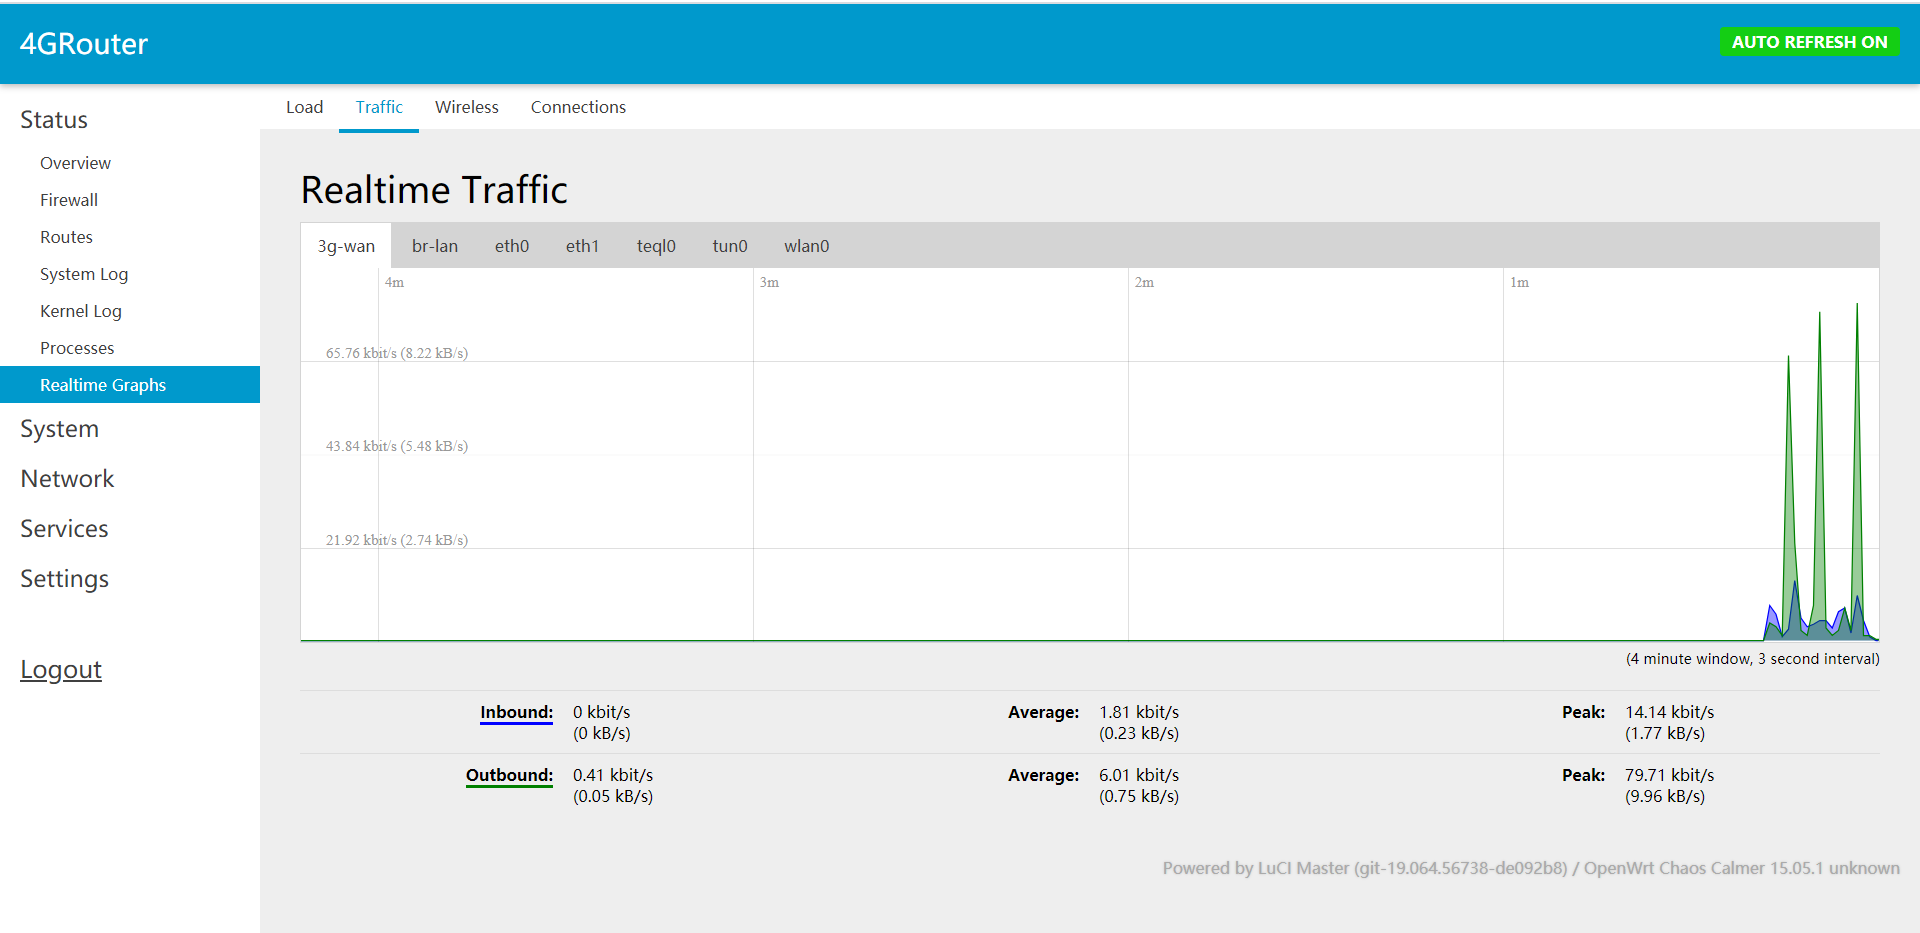
\includegraphics[totalheight=\tempheight]{immagini/interfacciar4g_traffic}
		\caption{Grafico del traffico}
	\end{subfigure}

	\vspace{1ex}

	\begin{subfigure}[b]{\textwidth}
		\centering%
		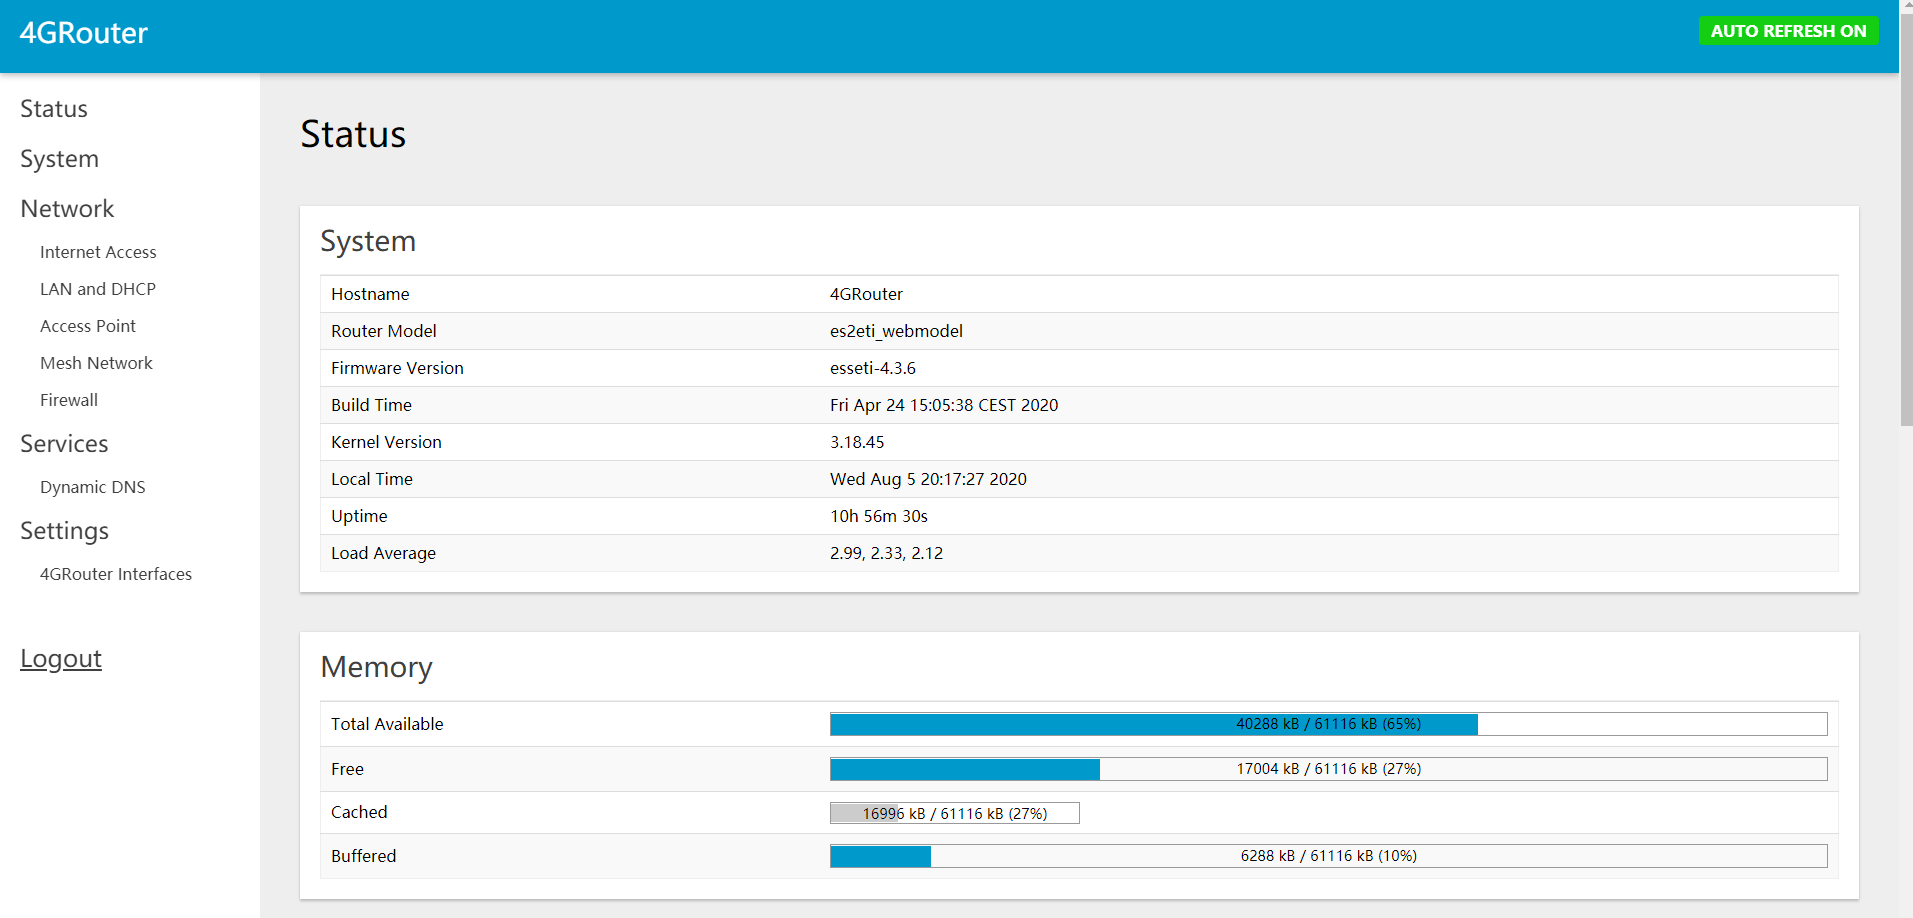
\includegraphics[totalheight=1.6\tempheight]{immagini/interfacciar4g_status}
		\caption{Schermata con stato riassuntivo}
	\end{subfigure}

\end{figure}

L'interfaccia web e' una versione personalizzata di \href{https://openwrt.org/docs/guide-user/luci/start}{Luci}.

Per semplicita' si fara' riferimento all'\textit{Esse-ti 4G.Router} chiamandolo semplicemente \it{Router}.

\subsection{VPS OVHCloud}

La VPS ha il solo vincolo di dover avere un'ip pubblico e una connessione a internet abbastanza veloce. Dovra' infatti sopportare un traffico simmetrico in upload / download.

Per la realizzazione della topologia e' stata selezionata una macchina una VPS del provider OVHCloud, con le seguenti caratteristiche:

\begin{itemize}
	\item 2 core virtuali
	\item 4Gb di memoria ram
	\item 80Gb di storage NVMe
	\item 500Mbps simmetrici di banda
	\item ipv4 pubblico
	\item Ubuntu 16.04
\end{itemize}

Per semplicita' si fara' riferimento alla \textit{VPS OVHCloud} come \it{Server}.

\subsection{Host domotico}

%TODO don't like
Per effettuare le varie operazioni di testing e' stato aggiunta \it{raspberry pi} che ha svolto il ruolo di "host domotico". Sono state fatti test con ping e iperf per testare che tutta la topologia sia stata configurata correttamente.


\subsection{Macchina del cliente}

%TODO da espandere
Deve poter essere una qualunque macchina, non ha vincoli di sistema operativo

Necessita di avere il client openvpn installato:

\begin{itemize}
	\item con sistema operativo Windows si deve scaricare l'eseguibile dal \href{https://openvpn.net/client-connect-vpn-for-windows/}{sito ufficiale}
	\item su linux e' sufficiente cercare nei repository ufficiali della distribuzione che si sta usando.
\end{itemize}


